% LAB 6: File I/O
% 
% CSE/IT 107: Introduction to Programming
% New Mexico Tech
% 
% Prepared by Russell White and Christopher Koch
% Spring 2015
\documentclass[11pt]{cselabheader}

%%%%%%%%%%%%%%%%%% SET TITLES %%%%%%%%%%%%%%%%%%%%%%%%%
\fancyhead[R]{Lab 6: File I/O}
\title{Lab 6: File I/O}

\begin{document}

\maketitle

\hrule
\begin{quotation}
``The danger that computers will become like humans is not as big as the danger
that humans will become like computers.'' (``Die Gefahr, dass der Computer so
wird wie der Mensch ist nicht so gro\ss, wie die Gefahr, dass der Mensch so wird
wie der Computer.'')
\end{quotation}
\begin{flushright}
--- Konrad Zuse
\end{flushright}

\begin{quotation}
	``First, solve the problem. Then, write the code.''
\end{quotation}
\begin{flushright}
	--- John Johnson
\end{flushright}

\begin{quotation}
``I don’t need to waste my time with a computer just because I am a computer
scientist.''
\end{quotation}
\begin{flushright}
--- Edsger W. Dijkstra
\end{flushright}

\hrule

\section{Introduction}
In previous labs, we taught you how to use functions, math, lists, strings, and
the like. We will combine all that in this lab and teach you how to interact
with files. This will lead us to do some exciting data analysis!

\section{File I/O}
Knowing how to work with files is important, since it lets us store and retrieve
data beyond the scope of the single execution of a program. To open a file for
reading or writing we will use the \lstinline{open} function. The following
example opens a file and writes ``Hello World'' to it.

\begin{python3code}
output_file = open("hello.txt", "w")

print("Hello World", file=output_file)
output_file.close()
\end{python3code}

The arguments to the \lstinline{open} function are, in order, the name of the
file to open and the mode in which to open the file. ``w'' means that the file
is to be opened in write mode. If the file does not exist, this will create the
file. If it does exist, then the contents of the file will be cleared in
preparation for the new ones.

Other options include ``a'', which is similar to ``w'' but will not clear the
contents of an existing file and will instead append the new data to the end,
and ``r'' which will read the file instead. If ``r'' is used and the file does
not exist, then an error will occur. The following code takes a filename as user
input, then prints out the entire contents of that file.

\begin{table}[!ht]
  \centering
  \begin{tabular}{ll}
    Mode & What it does \\
    \midrule
    a & Create file if does not exist, open file, append contents to the end \\
    w & Create file if does not exist, open file, write contents to the beginning
    of file \\
    r & Open file, permit reading only \\
  \end{tabular}
\end{table}

\begin{python3code}
filename = input("What file should be read? ")

input_file = open(filename, "r")
for line in input_file:
  print(line, end="")

input_file.close()
\end{python3code}

The additional concepts introduced in these examples are:

\begin{itemize}
\item The \lstinline{print} function can have an additional ``file'' parameter
  passed to it to allow writing to a file. This causes it to send its output to
  the file rather than the screen, though otherwise it performs identically.

\item The \lstinline{print} function has an additional optional ``end''
  parameter. This allows you to specify what should be printed after the main
  string given to it. This is important because it defaults to \lstinline{"\n"},
  which causes a newline after every print statement. By changing ``end'' to
  \lstinline{""} we prevent a newline from being added after every line of the
  file is printed. This is because each line in the file already has a newline
  at the end of it, so we don't need \lstinline{print} to add its own.

\item \lstinline{.close()} is used to properly tell Python that you are done
  with a file and close your connection to it. This isn't \emph{strictly}
  required, but without it you risk the file being corrupted or other programs
  being unable to access that file.

\item When reading from a file, Python can use a \lstinline{for} loop to go
  through each line in sequence. This works identically to if you think of the
  file as a list with every line being a different element of the list. The
  entirety of the file can also be read into a single string using the
  \lstinline{.read()} function.

\begin{pyconcode}
>>> input_file = open("test.py", "r")
>>> contents = input_file.read()
>>> print(contents)
filename = input("What file should be read? ")

input_file = open(filename, "r")
for line in input_file:
  print(line, end="")

input_file.close()
\end{pyconcode}

\item \lstinline{.readlines()} can be used to read all of a file at once, though
  it splits the file into a list. Each element of the list will be one line of
  the file being read.
\end{itemize}


\subsection{Error Handling}
If you try to open a file that does not exist for reading, Python will display
an error message:

\begin{pyconcode}
>>> open("not_a_file.txt", "r")
Traceback (most recent call last):
  File "<pyshell#0>", line 1, in <module>
  open("not_a_file.txt", "r")
FileNotFoundError: [Errno 2] No such file or directory: 'not_a_file.txt'
\end{pyconcode}

In this case, the error is \lstinline{FileNotFoundError}. Normally having an
error occur will end your program, but we can use \lstinline{try-except} in
order to perform a special action in case of an error. The following program
uses this to display an error message rather than crashing.

\begin{python3code}
filename = input("What file should be read? ")

try:
  input_file = open(filename, "r")
  for line in input_file:
    print(line, end="")

  input_file.close()
except FileNotFoundError:
  print("Could not find file {}.".format(filename))
\end{python3code}

If you wish to catch an error, check the error message for the name of the error
that you need to catch with your \lstinline{except} statement. If the specified
error does not occur inside the \lstinline{try} block, then the
\lstinline{except} block will be skipped. A single \lstinline{try} block can
have several \lstinline{except} statements following it for catching multiple
types of errors.

%\section{Recursion}
\pagebreak
\section{Instantiating Turtles}
Similarly to being able to open multiple files, we can also create multiple
turtles to draw more complex designs. This is done using the
\lstinline{turtle.Turtle()} function. This function returns a turtle object,
which we can call every other normal turtle function on.

\begin{python3code}
import turtle

first = turtle.Turtle()
second = turtle.Turtle()

first.forward(50)
second.forward(50)
first.left(90)
second.right(90)
first.forward(50)
second.forward(50)
first.right(90)
second.left(90)
first.forward(50)
second.forward(50)
\end{python3code}

\begin{figure}[h]
  \centering
  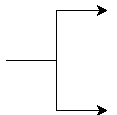
\includegraphics[width=1.0in]{img/turtle_prong}
\end{figure}

If we add a group of turtles to a list, we can easily apply the same commands to all of them, as in this example:

\begin{python3code}
import turtle

turtles = []
first = turtle.Turtle()
first.speed(0)
turtles.append(first)

second = turtle.Turtle()
second.speed(0)
second.right(90)
turtles.append(second)

third = turtle.Turtle()
third.speed(0)
third.right(180)
turtles.append(third)

fourth = turtle.Turtle()
fourth.speed(0)
fourth.right(270)
turtles.append(fourth)

for i in range(200):
    for turt in turtles:
        turt.forward(i/5)
        turt.left(10)
\end{python3code}

\begin{figure}[h]
  \centering
  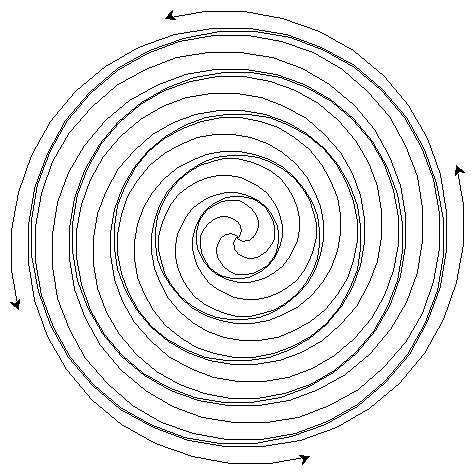
\includegraphics[width=2.0in]{img/fancy_spiral}
\end{figure}

\pagebreak
\section{Exercises}
\label{sec:ex}

\begin{ex}[save.py] Write a program that takes in a filename, then takes in
  a series of lines of input until a blank line is entered, writing each line to
  the file with the given name. After the blank line is entered, properly close
  the file before ending the program.  
\end{ex}

\begin{ex}[word\_count.py] Write a program that
  takes in a filename and string as input. Then print how many times that string
  appears inside the chosen file. If the file does not exist, continue asking
  for a filename until one is given that exists. Use your source code file as
  test input.
\end{ex}

\begin{ex}[navigate3.py] Modify navigate.py so that, rather than take instructions
    from the command line, it reads from a file (specified by user input) to
    determine what the turtle will do. Additionally, you will be adding the
    ``split'' command. This command will use instantiation of new turtles in order
    to draw multiple lines at once. Every new command will apply to every turtle
    that currently exists. The file will have on instruction per line. The
    possible instructions are:

    \begin{description}
      \item[forward X] Move all turtles forward X.
      \item[left X] Turn all turtles X degrees to the left.
      \item[right X] Turn all turtles X degrees to the right.
      \item[split X] Split all turtles into new turtles. Each new turtle will be turned X degrees to the right.
    \end{description}

    In order to properly implement split, you will probably need to look up the
    turtle functions \lstinline{.position()}, \lstinline{.setposition()},
    \lstinline{.setheading()}, \lstinline{.heading()}, \lstinline{.penup()}, and
    \lstinline{.pendown()}. Turtle documentation is available at
    \url{https://docs.python.org/3/library/turtle.html}.

    You will also likely use the \lstinline{.split()} command when getting input, which splits a single string into an array around the string's spaces.
    \begin{pyconcode}
>>> print("this is a phrase".split())
['this', 'is', 'a', 'phrase']
>>> print("hi,hi,hi".split(",")
['hi', 'hi', 'hi']
    \end{pyconcode}

    \emph{Suggestion:} Split each command into a different function to help keep their logic separate.

    Sample Input File:
    \begin{python3code}
forward 50
left 20
split 40
forward 50
left 20
split 40
forward 50
left 20
split 40
forward 50
left 20
split 40
forward 50
left 20
    \end{python3code}

    Sample Output
    \begin{center}
      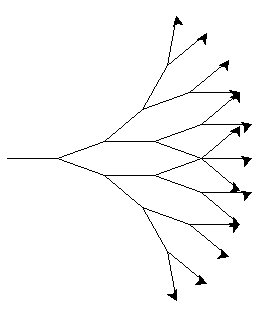
\includegraphics[width=1.0in]{img/nav3_example}
    \end{center}
  \end{ex}

  \begin{ex}[states.py]
    Look at the file \texttt{states.csv} given. It has the following columns, in
    the following order:
    \begin{itemize}
      \item State name
      \item Population in thousands
      \item Life expectation in years
      \item Murder rate per 1,000,000 people
      \item High school graduation rate
      \item Area in square miles
    \end{itemize}

    Write a program that reads in all this data to a list of lists and then
    \emph{write a function} for each of the following:
    \begin{itemize}
      \item Find the murder rate per 1,000,000 people for the United States.
      \item Find the murder rate per square mile for each state and then the
        United States.
      \item Find the high school graduation rate per area for each state.
      \item Find the total area of the United States.
      \item Find the population density (population per area) of the United
        States.
    \end{itemize}

    Print the per state information in a table.
  \end{ex}

\pagebreak
\section{Submitting}

You should submit your code as a tarball. It should contain all files
used in the exercises for this lab. The submitted file should be named
\begin{center}
  \texttt{cse107\_firstname\_lastname\_lab5.tar.gz}
\end{center}

\begin{center}
  \textbf{Upload your tarball to Canvas.}
\end{center}

\listoftheorems


\end{document}
